% для компиляции в lualatex!!
\documentclass[12pt, a4paper]{article}
\usepackage[english,russian]{babel}
\usepackage[warn]{mathtext}
%\usepackage[T2A]{fontenc}
%\usepackage[utf8]{inputenc}

\usepackage{xecyr} % Продукт Вашего покорного слуги ;)

\setmainfont{DejaVu Serif}

\usepackage{color}
\usepackage{amssymb,amsmath}
\usepackage{graphicx}
\usepackage{multicol}

\textheight=24cm           % высота текста
\textwidth=16cm            % ширина текста
\oddsidemargin=0pt         % отступ от левого края
\topmargin=-1.5cm          % отступ от верхнего края
\parindent=24pt            % абзацный отступ
\parskip=0pt               % интервал между абзацами
\tolerance=2000            % терпимость к "жидким" строкам
\flushbottom               % выравнивание высоты страниц
%\def\baselinestretch{1.5} % печать с большим интервалом

%\title{}
%\author{\copyright~~С.А.~Назарова \thanks{e-mail:~sophia.nazarova@gmail.com}}
%\date{}

\begin{document}

%\maketitle

%Эстуарий Лувеньги


\begin{figure}[h]

\begin{multicols}{3}
\hfill
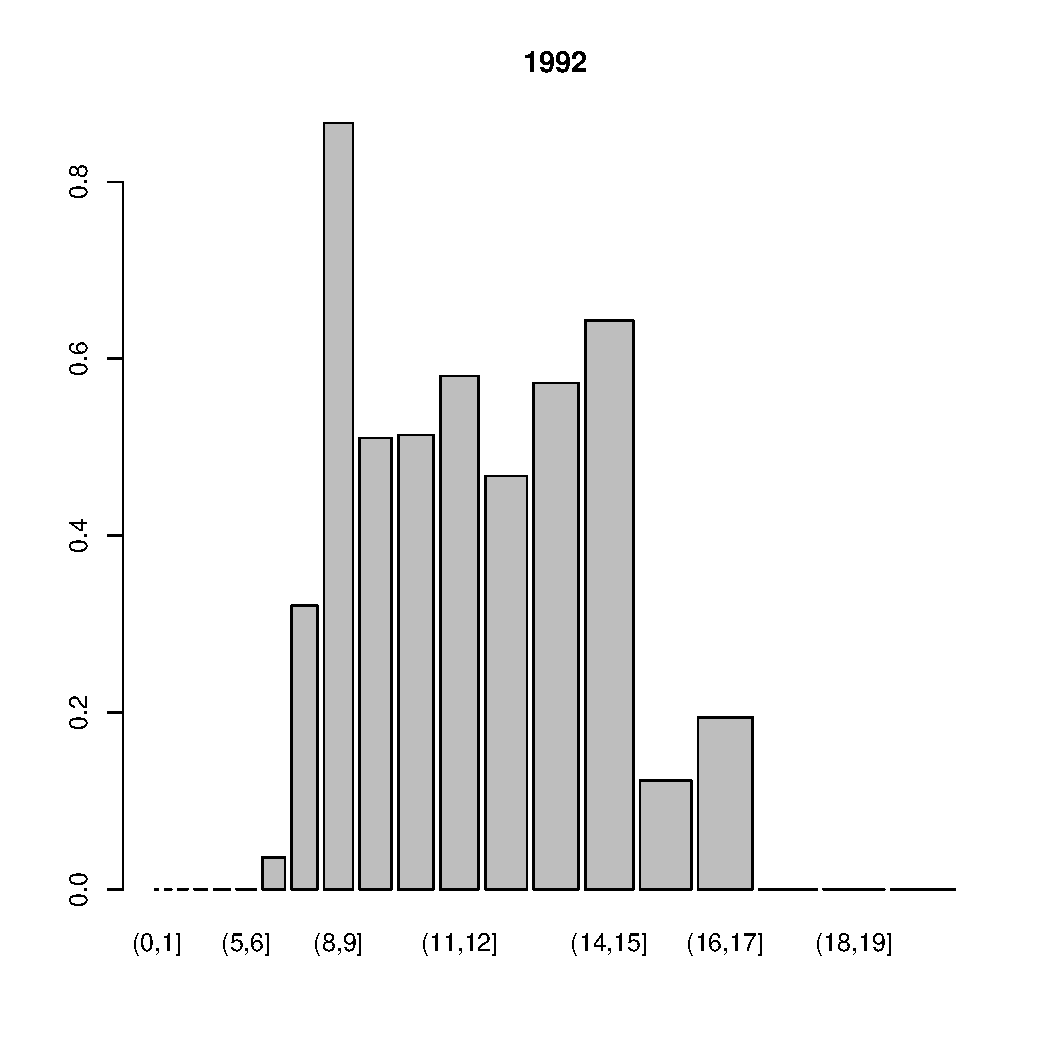
\includegraphics[width=65mm]{../White_Sea/Estuatiy_Luvenga/sizestr_percents_1992_.pdf}
\hfill
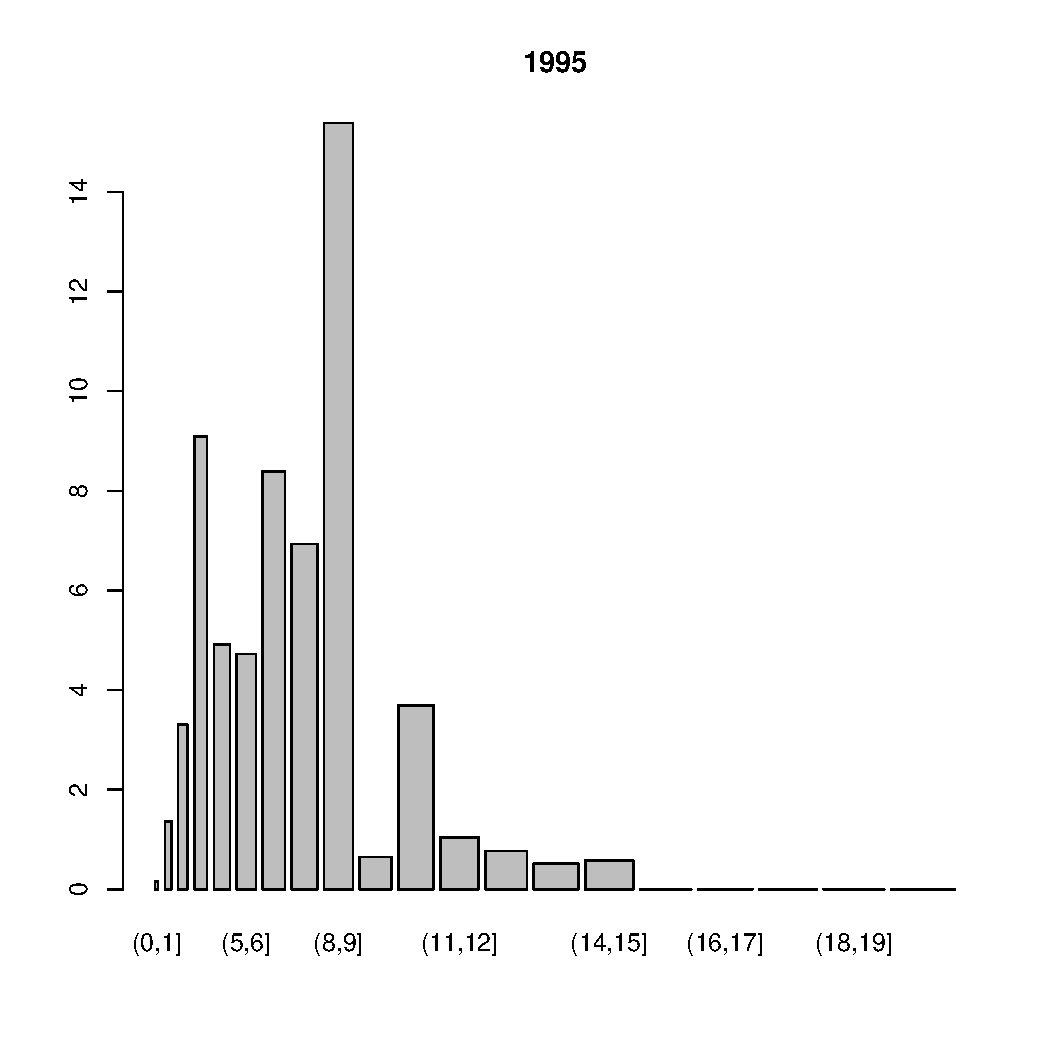
\includegraphics[width=65mm]{../White_Sea/Estuatiy_Luvenga/sizestr_percents_1995_.pdf}

\hfill
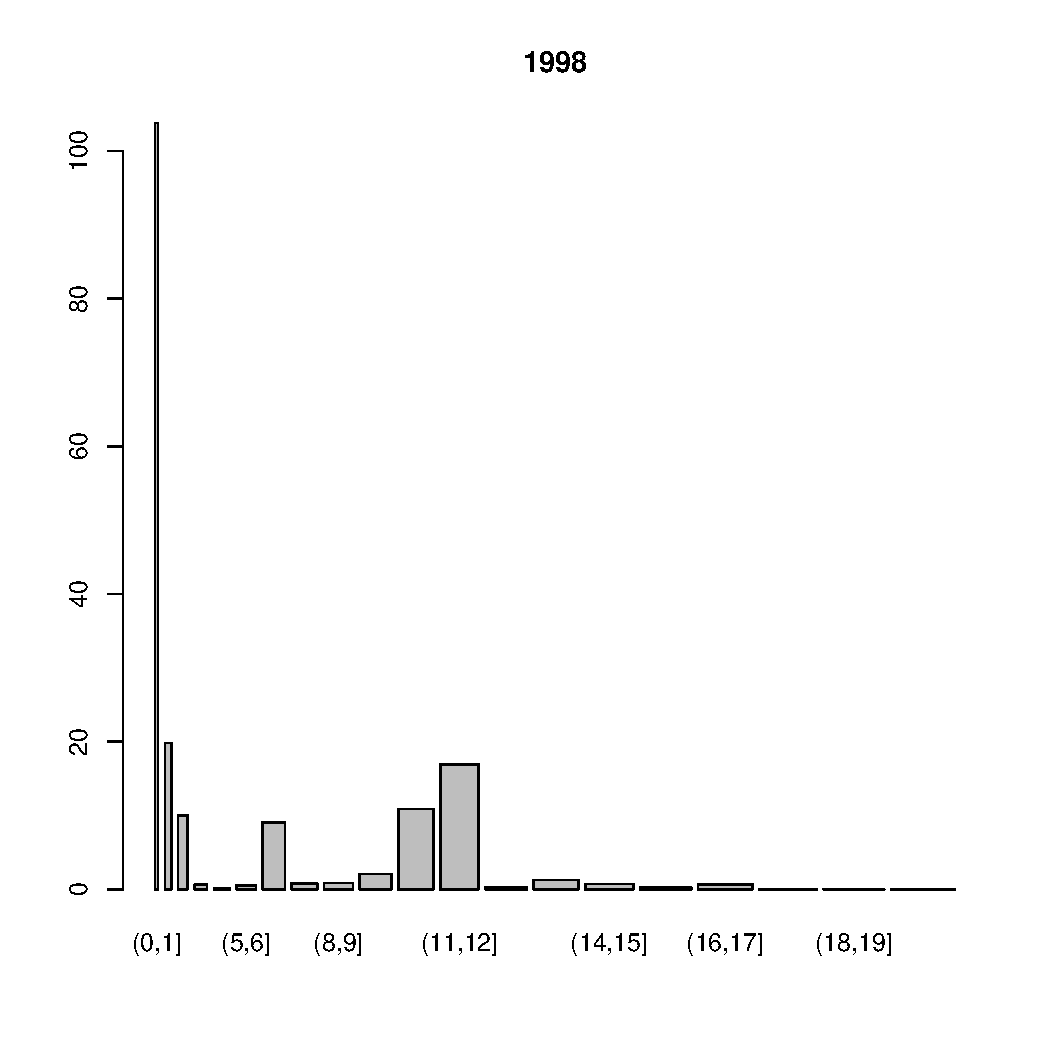
\includegraphics[width=65mm]{../White_Sea/Estuatiy_Luvenga/sizestr_percents_1998_.pdf}

\end{multicols}

%\smallskip


\begin{multicols}{3}
\hfill
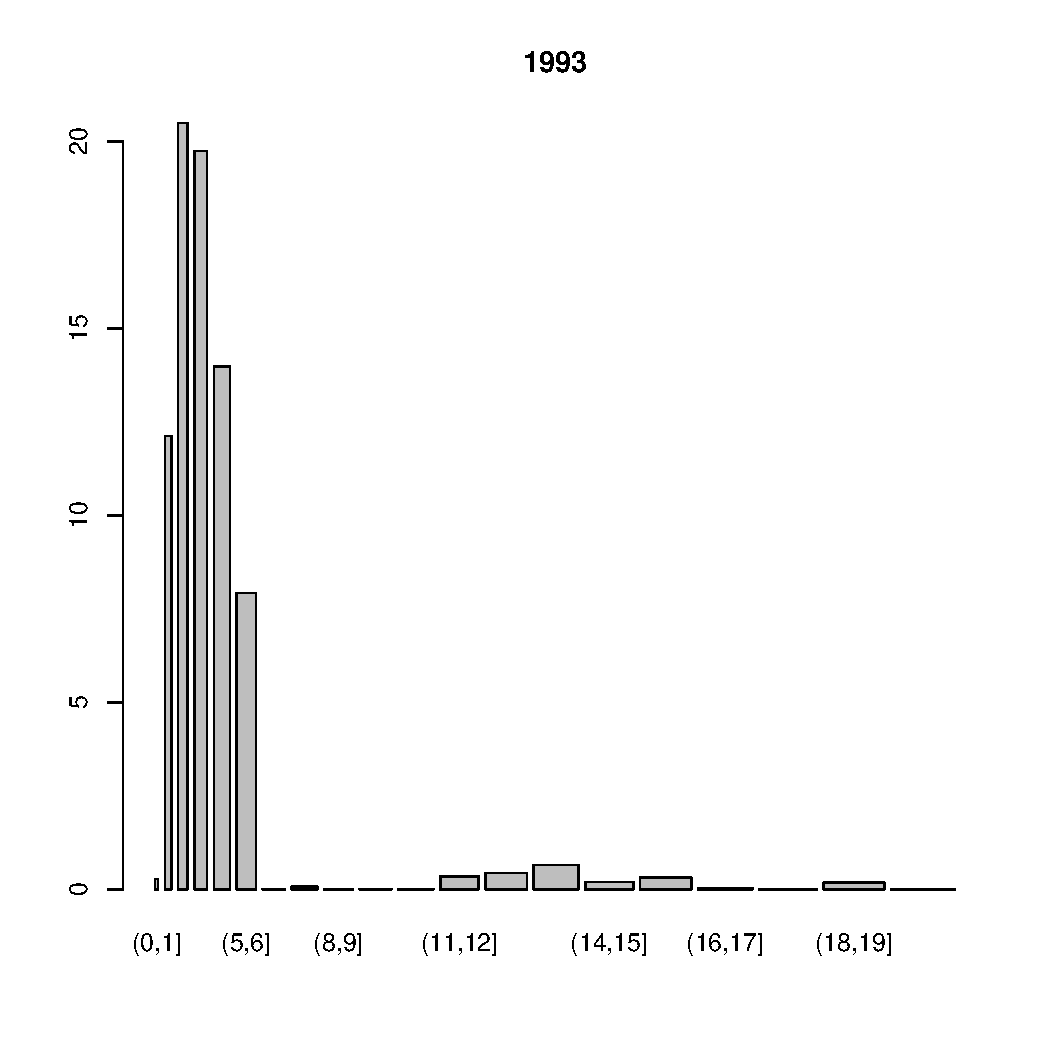
\includegraphics[width=65mm]{../White_Sea/Estuatiy_Luvenga/sizestr_percents_1993_.pdf}
\hfill
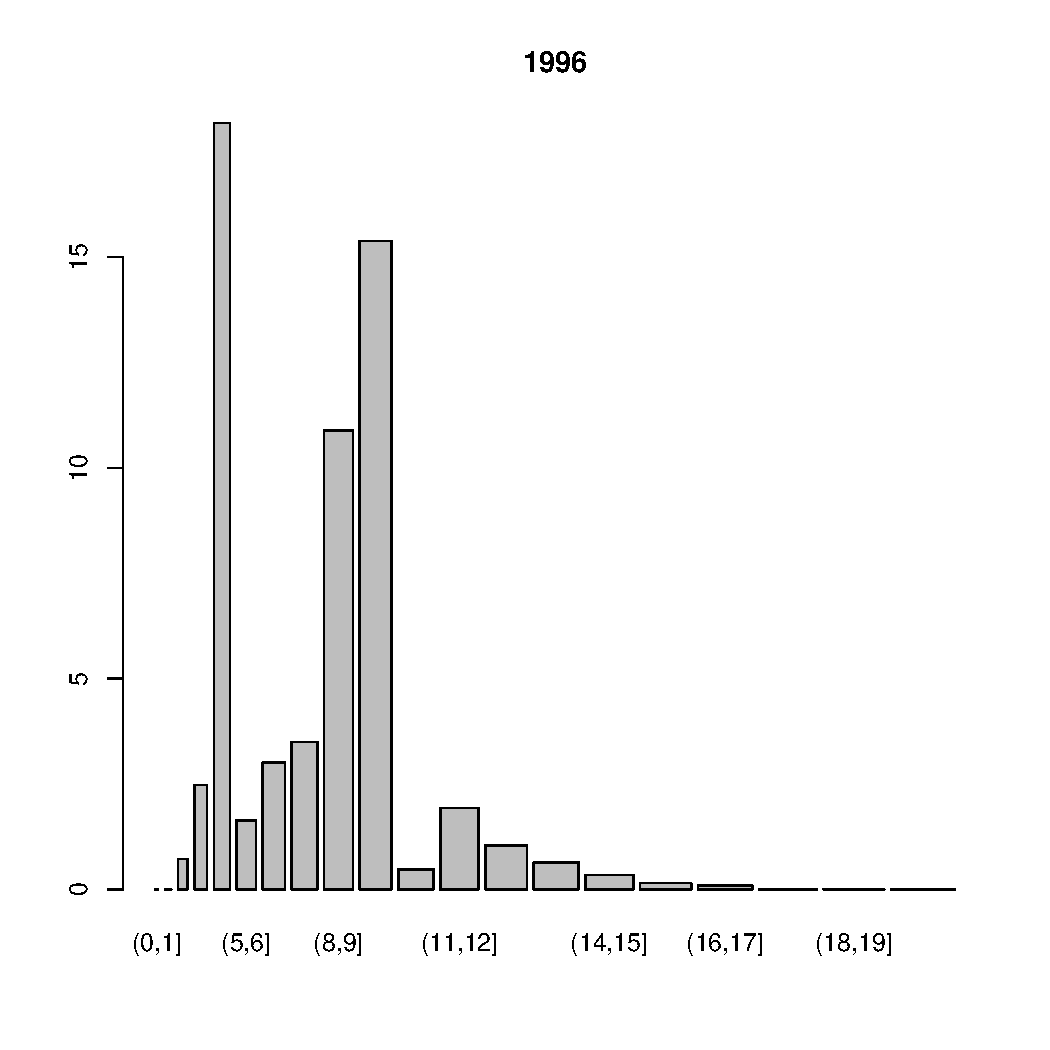
\includegraphics[width=65mm]{../White_Sea/Estuatiy_Luvenga/sizestr_percents_1996_.pdf}
\hfill
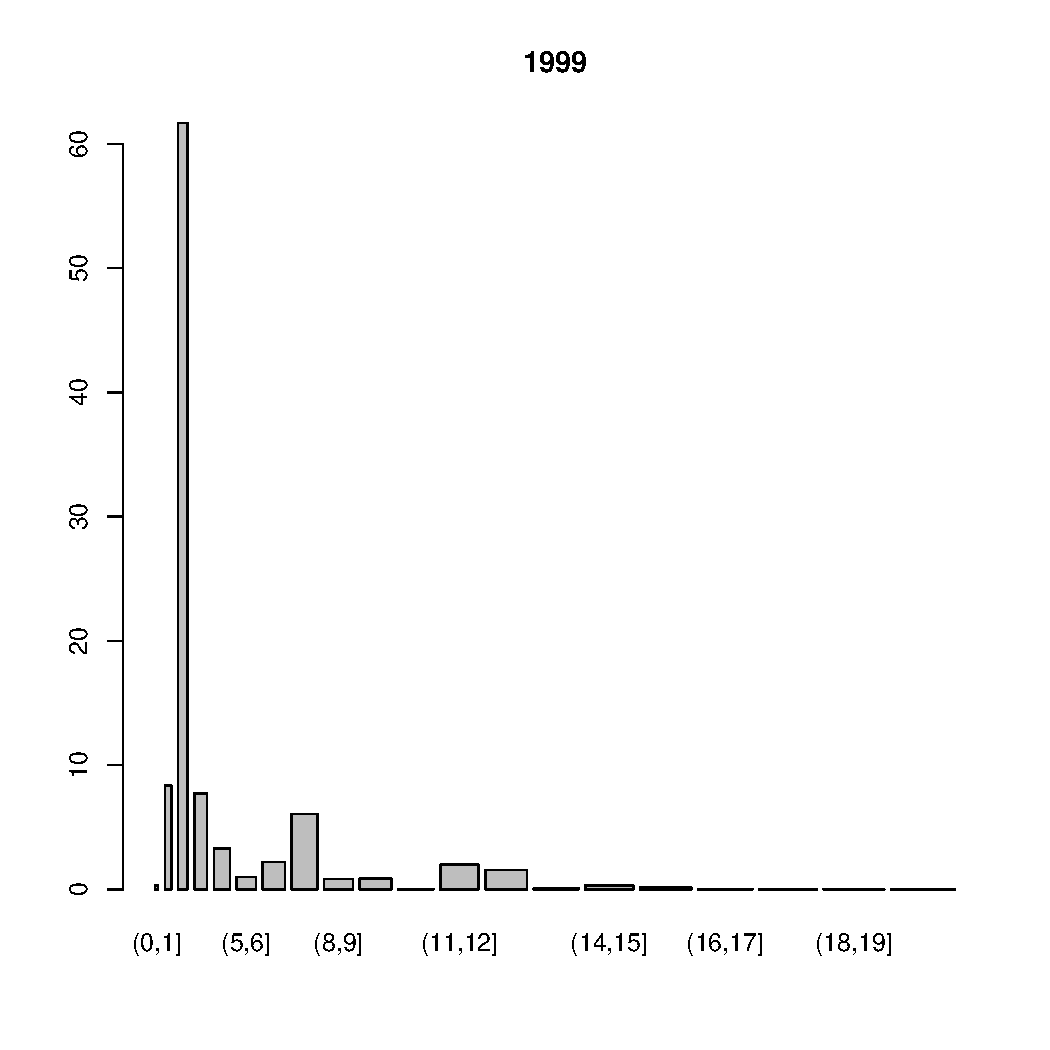
\includegraphics[width=65mm]{../White_Sea/Estuatiy_Luvenga/sizestr_percents_1999_.pdf}

\end{multicols}

%\smallskip

\begin{multicols}{3}
\hfill
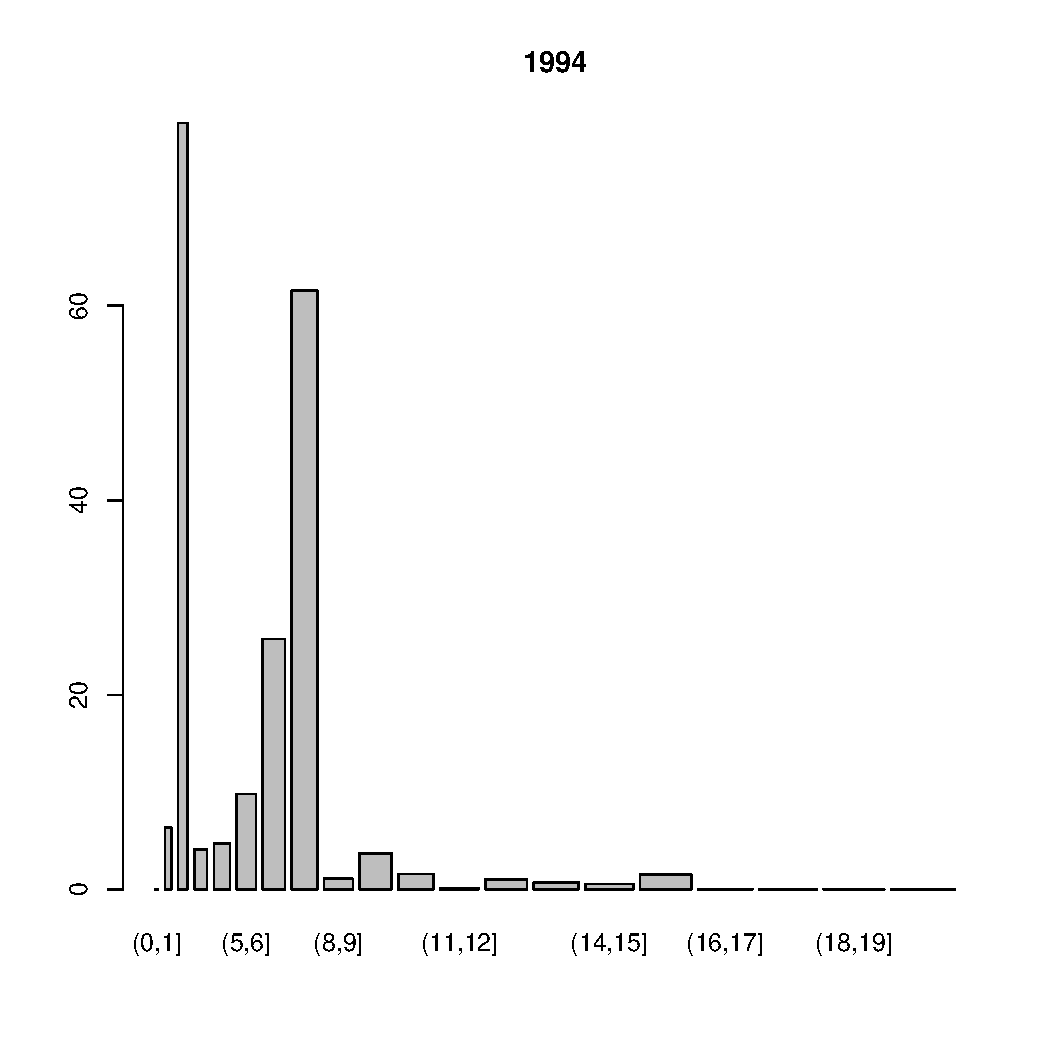
\includegraphics[width=65mm]{../White_Sea/Estuatiy_Luvenga/sizestr_percents_1994_.pdf}
\hfill
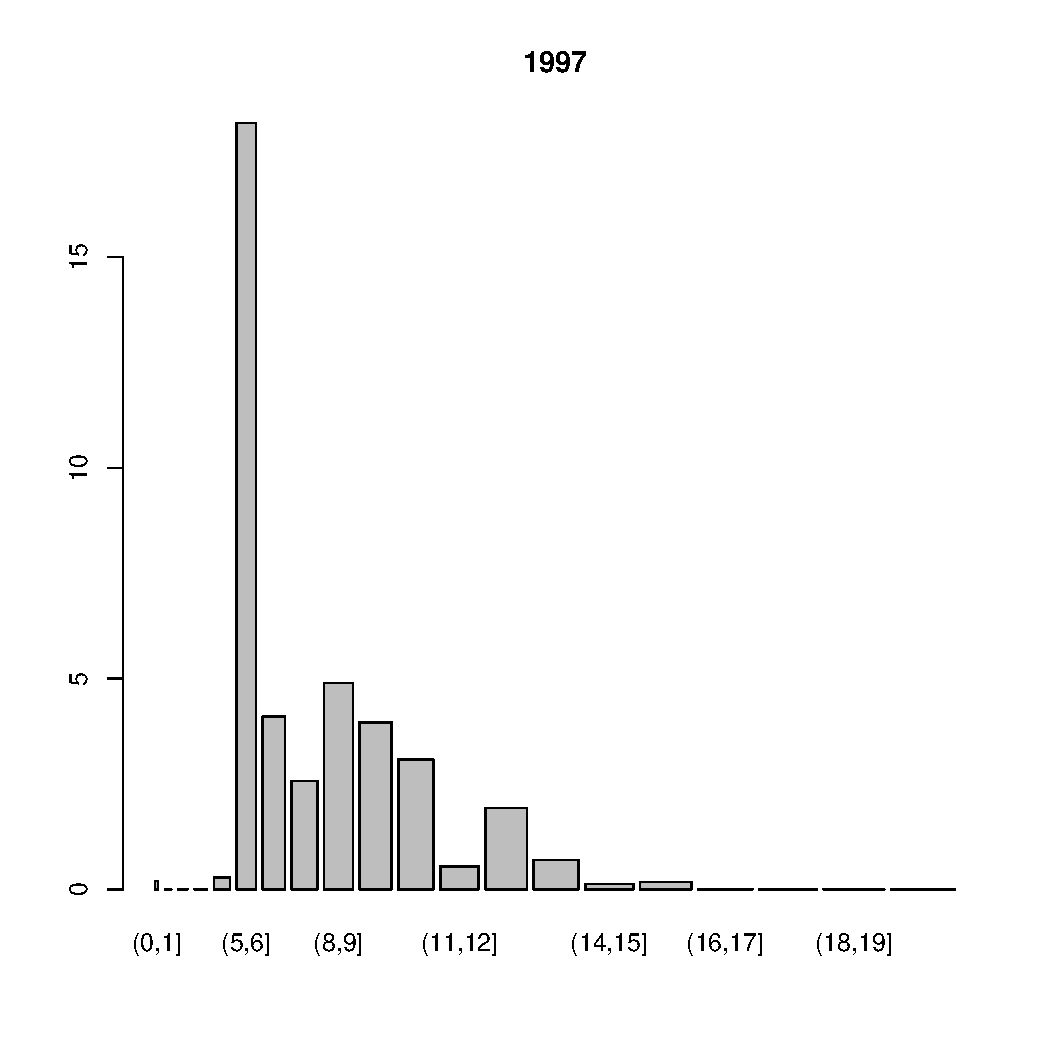
\includegraphics[width=65mm]{../White_Sea/Estuatiy_Luvenga/sizestr_percents_1997_.pdf}
\hfill
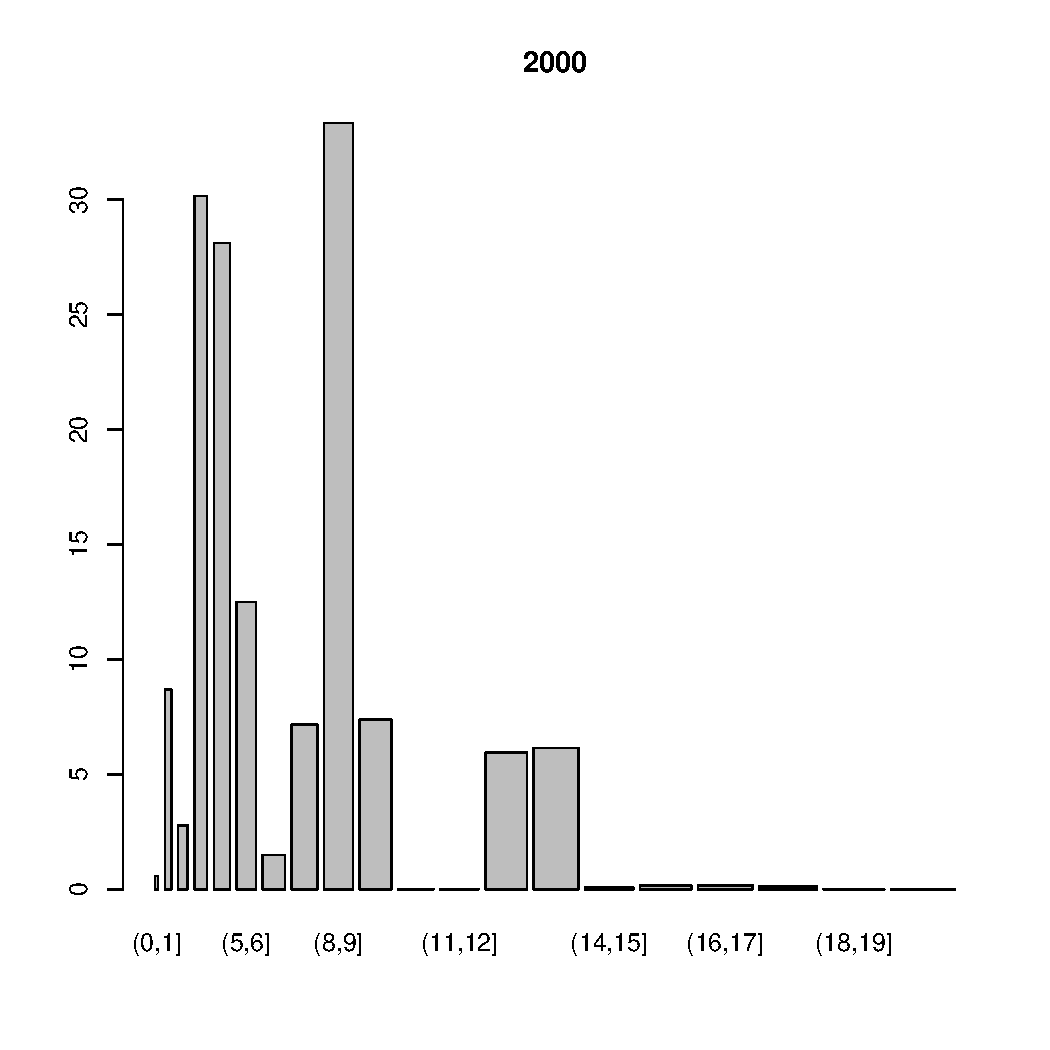
\includegraphics[width=65mm]{../White_Sea/Estuatiy_Luvenga/sizestr_percents_2000_.pdf}
\end{multicols}

%\smallskip


\caption{Размерная структура {\it Macoma balthica} в СГЛ эстуария р. Лувеньги.}
\label{ris:size_str_estuary_Luv}

По оси ординат --- доля особей в процентах от общей численности
\end{figure}


\begin{figure}[h]

\begin{multicols}{3}
\hfill
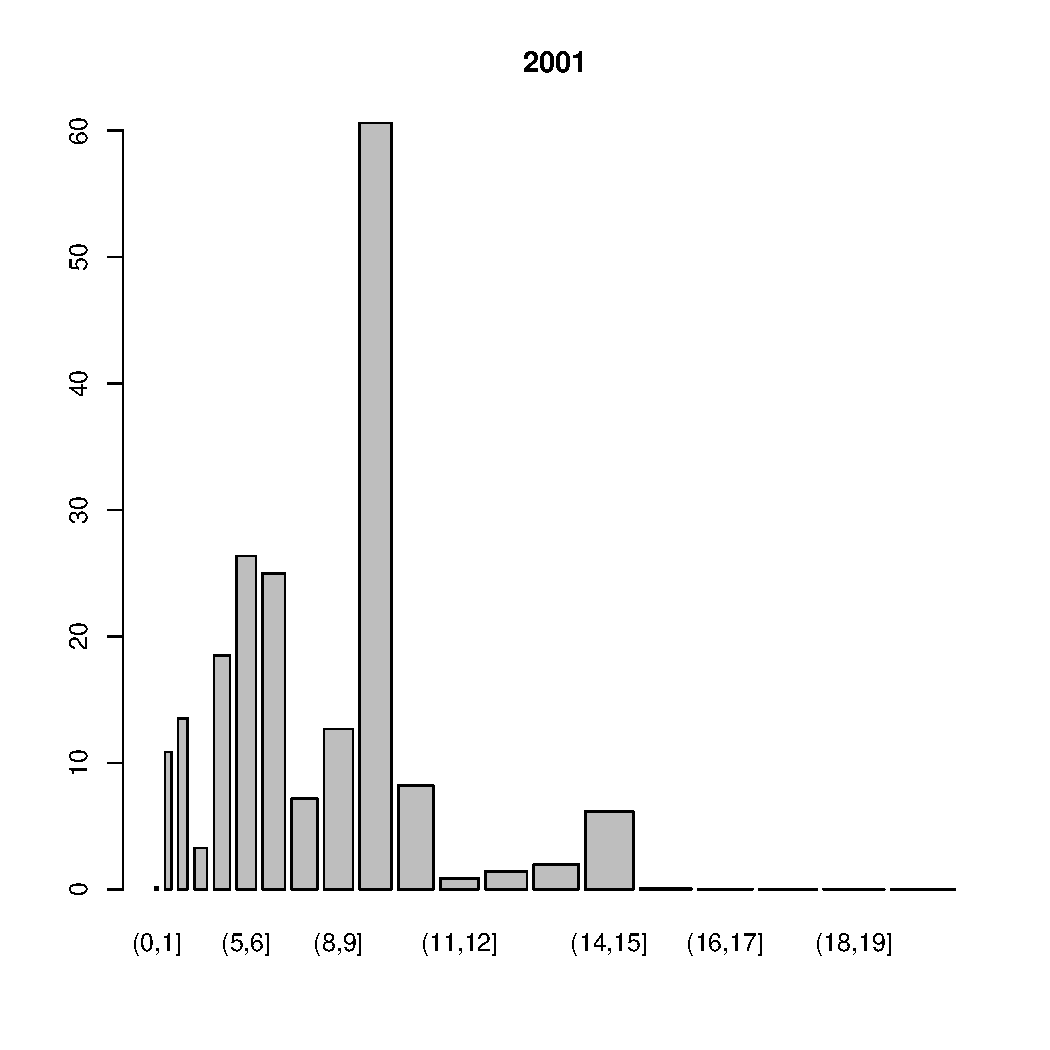
\includegraphics[width=65mm]{../White_Sea/Estuatiy_Luvenga/sizestr_percents_2001_.pdf}
\hfill
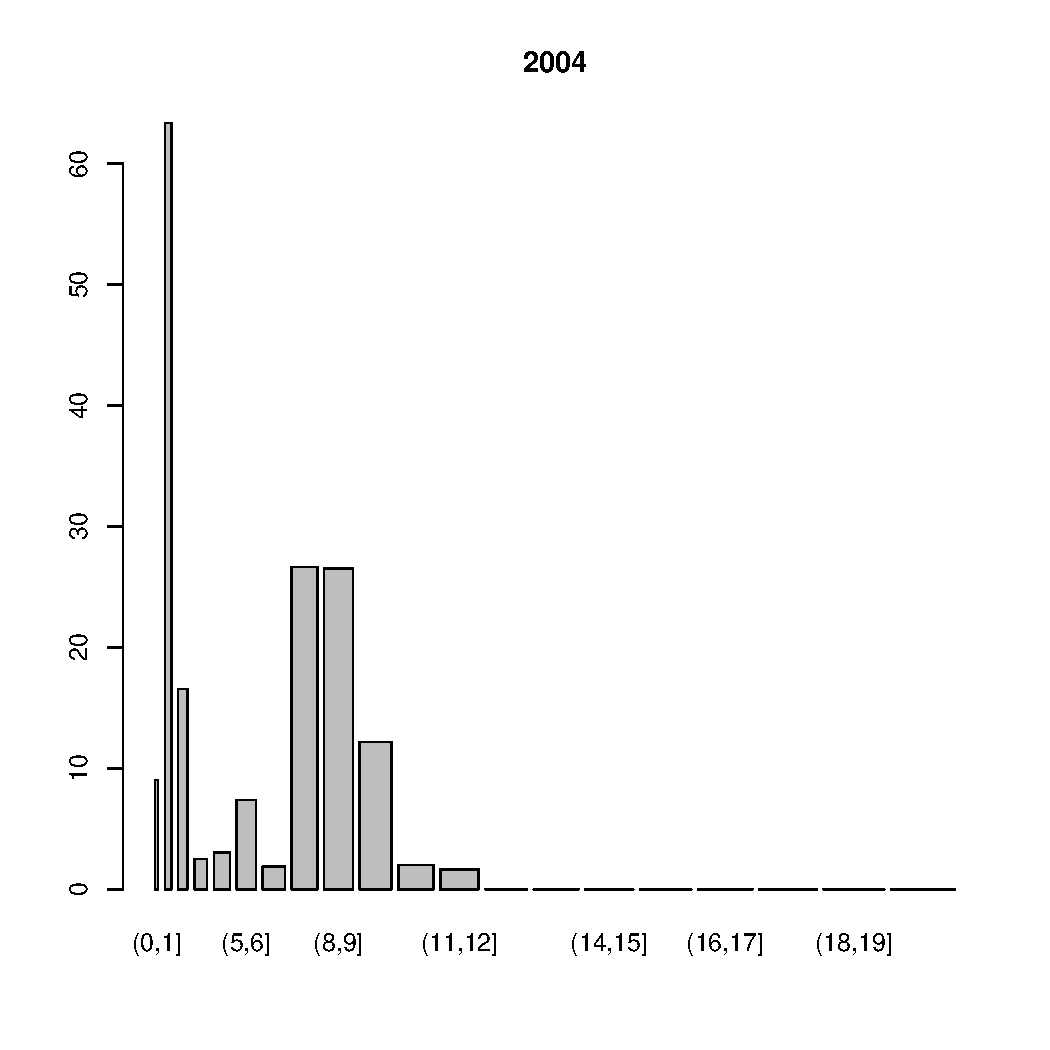
\includegraphics[width=65mm]{../White_Sea/Estuatiy_Luvenga/sizestr_percents_2004_.pdf}
\hfill
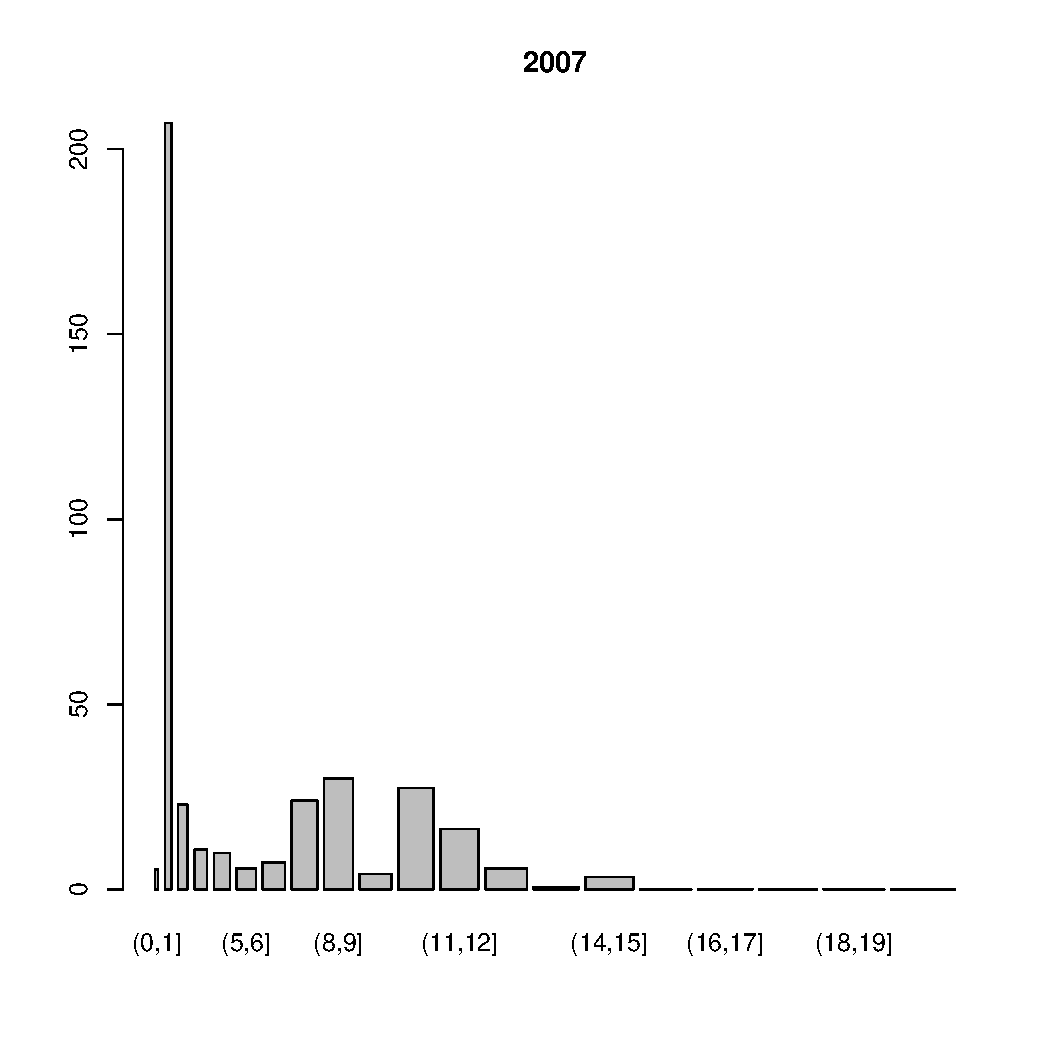
\includegraphics[width=65mm]{../White_Sea/Estuatiy_Luvenga/sizestr_percents_2007_.pdf}
\end{multicols}

\begin{multicols}{3}
\hfill
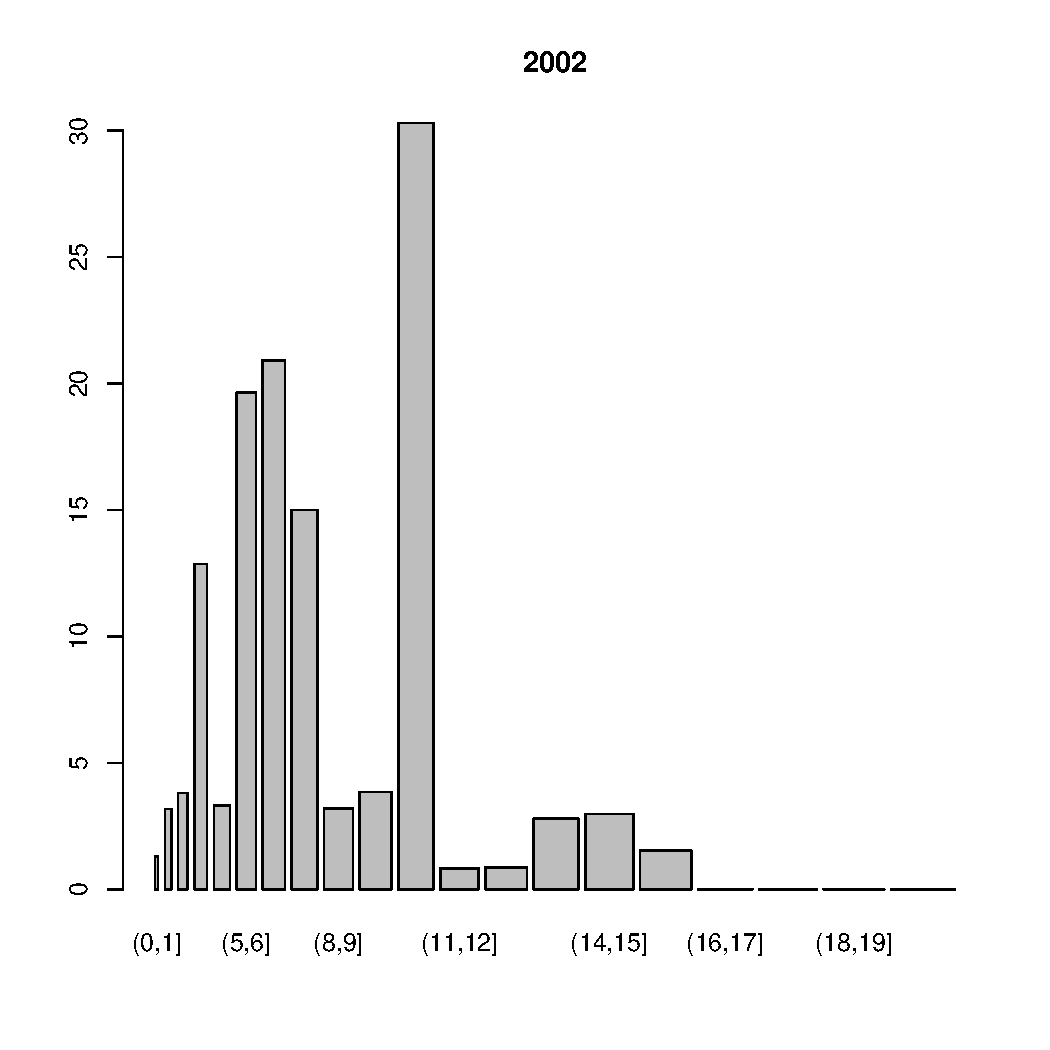
\includegraphics[width=65mm]{../White_Sea/Estuatiy_Luvenga/sizestr_percents_2002_.pdf}
\hfill
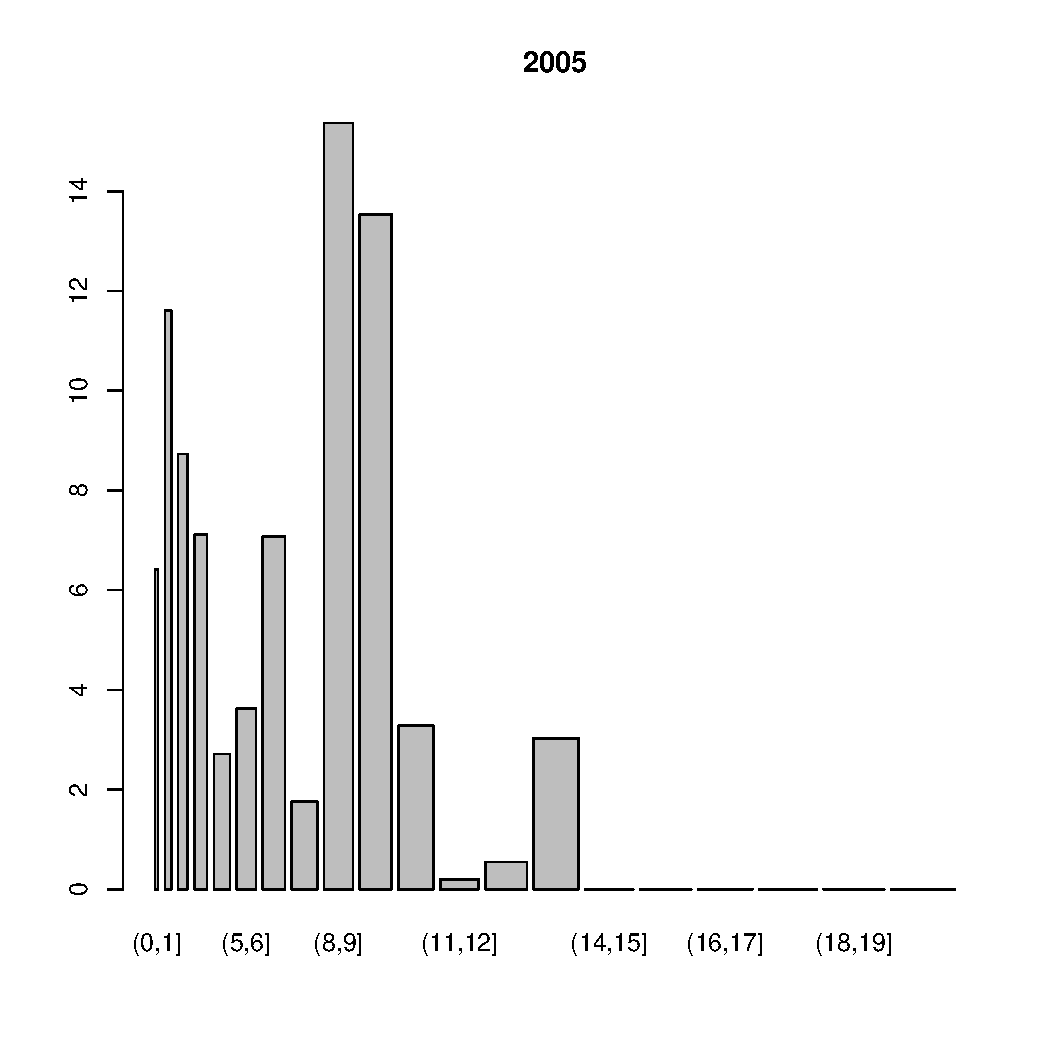
\includegraphics[width=65mm]{../White_Sea/Estuatiy_Luvenga/sizestr_percents_2005_.pdf}
\hfill
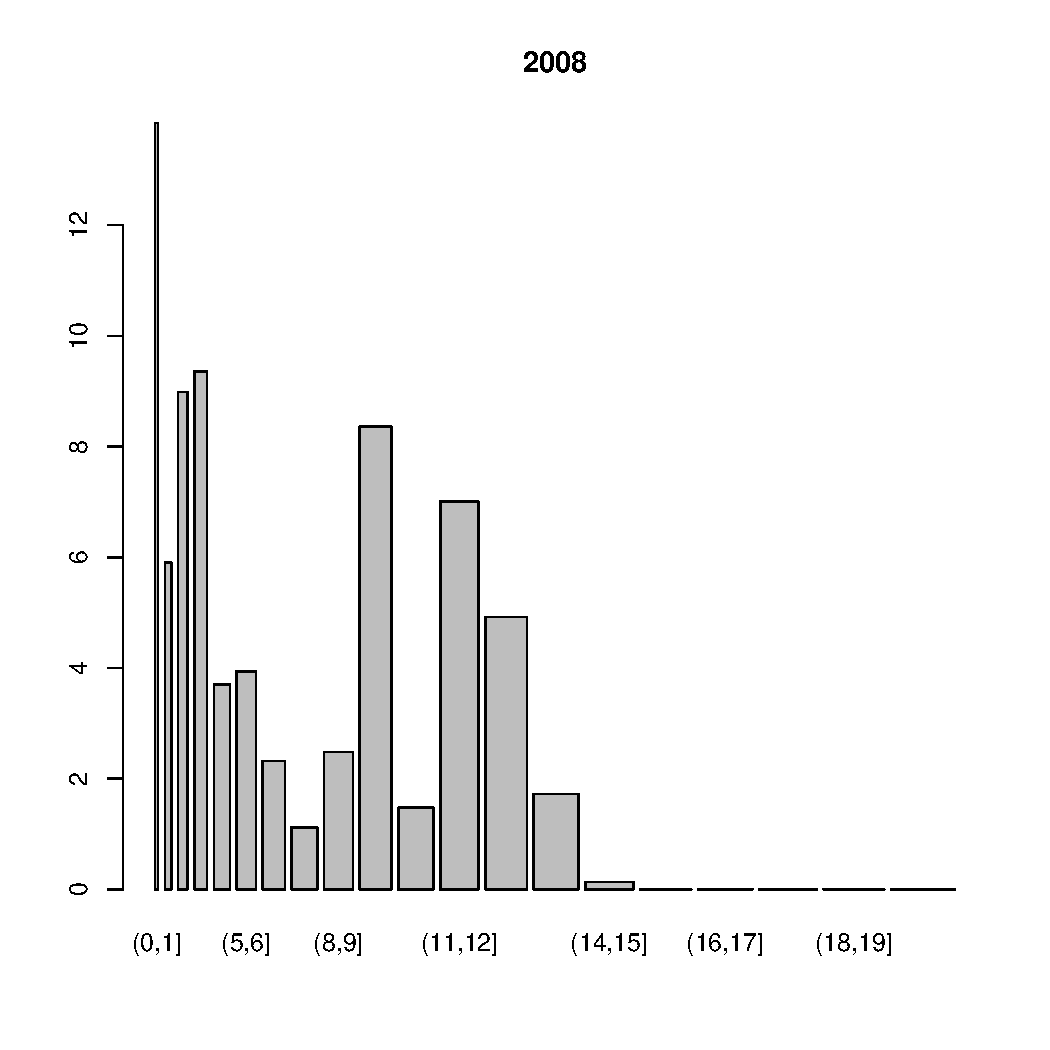
\includegraphics[width=65mm]{../White_Sea/Estuatiy_Luvenga/sizestr_percents_2008_.pdf}
\end{multicols}

%\smallskip


\begin{multicols}{3}
\hfill
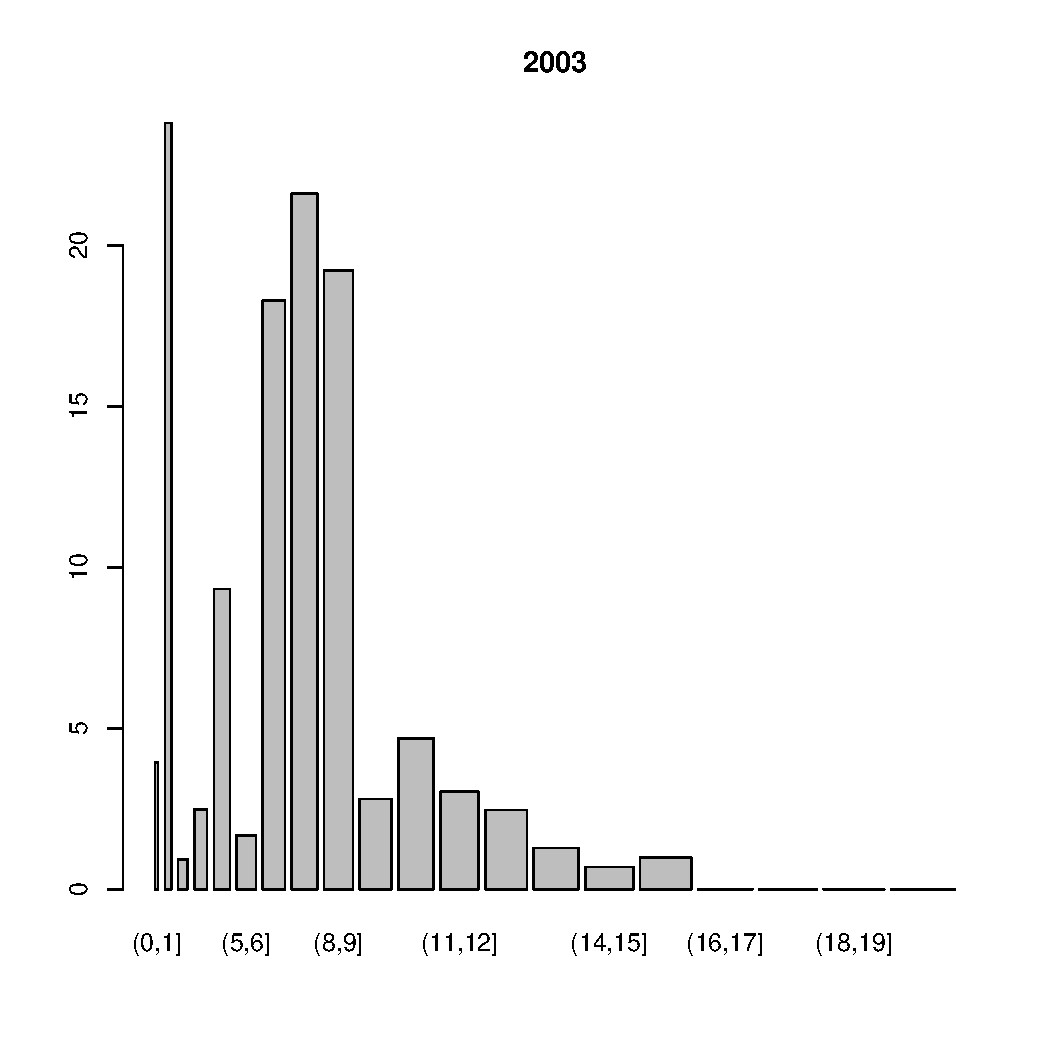
\includegraphics[width=65mm]{../White_Sea/Estuatiy_Luvenga/sizestr_percents_2003_.pdf}
\hfill
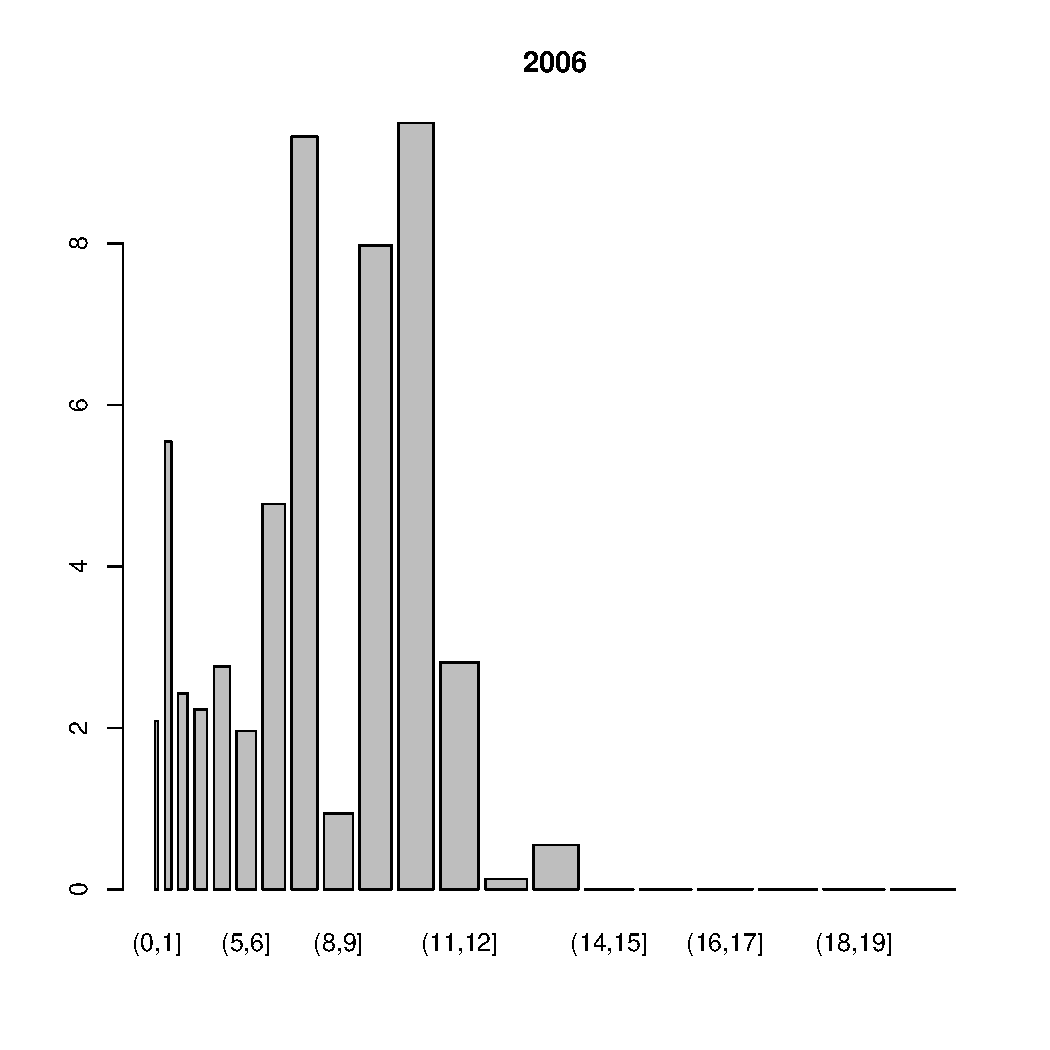
\includegraphics[width=65mm]{../White_Sea/Estuatiy_Luvenga/sizestr_percents_2006_.pdf}
\hfill
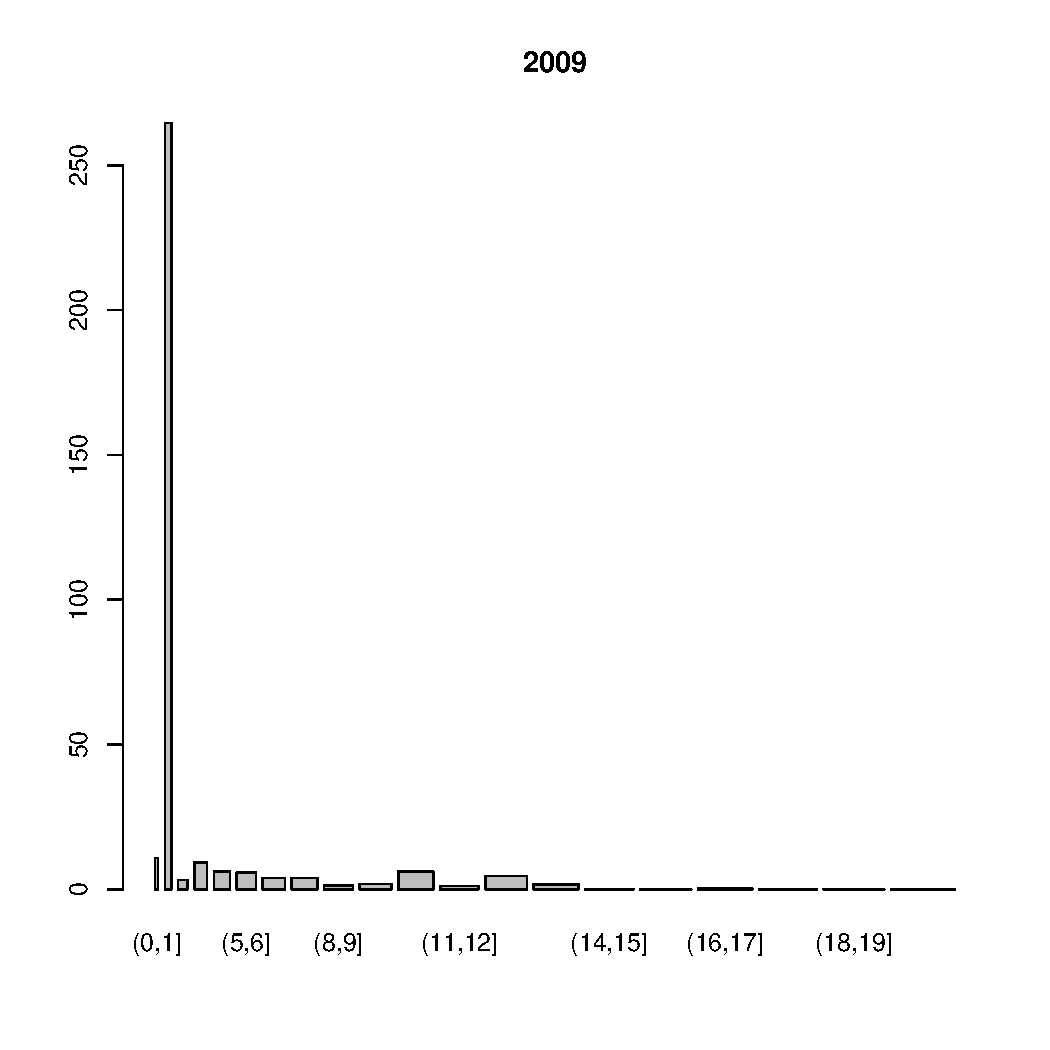
\includegraphics[width=65mm]{../White_Sea/Estuatiy_Luvenga/sizestr_percents_2009_.pdf}
\end{multicols}

%\smallskip


%\caption{Размерная структура {\it Macoma balthica} в СГЛ эстуария р. Лувеньги}
%\label{ris:size_str_estuaty_Luv}
\begin{center}
Рис. \ref{ris:size_str_estuary_Luv} (продолжение). Размерная структура {\it Macoma balthica} в СГЛ эстуария р. Лувеньги\\
По оси ординат --- доля особей в процентах от общей численности.

\end{center}
\end{figure}
\end{document}
